%Theory --- important this is clear as possible
% first trial includes a lot of figures as it makes it clearer to me

\section{Theory}

\section{Key Terms}

\subsection{Citizen Science}
Citizen science can take many varied forms, but the common factor is the involvement of volunteers. People who chose to use their time to assist in science who are not paid for their time \cite{pocock_choosing_2014}. Considering \cite{tweddle_guide_2012} the participation of volunteers was deemed critical for this project and will assist in the overall aims. This is because the data required would not be accessible using other techniques and the research was designed to improve the awareness of sea level extremes in Trondheim. The volunteers, who will henceforth be referred to as subjects, contributions were respected and the impact of their time by the research was minimised. After this project submission the results will be published in an accessible form for those subjects who are interested. This is inline with the guidelines for citizen science set out by \cite{tweddle_guide_2012} The data management plan and ethics guidance were created inline with \cite{nesh_guidelines_2022} and \cite{nsd_norsk_nodate}.


\subsection{Stakeholders}
The stakeholders primarily considered during this project are the people who live commute or work in coastal Trondheim. This was decided using \cite{reed_stakeholder_nodate} as a back up for a very basic stakeholder analysis. Other stakeholders considered are people with attachment to the research sites as well as well as planners and policy makers. Creating a full understanding prior to research of who was a stakeholder was not a priority as the primary research method relies upon stakeholders to self identify by choosing to take part in this research. However, targeting of subjects utilising the decided upon stakeholders was done. 

\paragraph{}
The stakeholders identity is a key part of the research. The nature of stakeholder participation during this project was limited to communication and consultation according to Rowe and Frower 2000 in \cite{reed_stakeholder_nodate}. How these stakeholders are categorised was predominately top down as community membership of certain groups were targeted with the ability to identify as these groups during the survey \cite{reed_stakeholder_nodate}. However, there was also bottom up stakeholder identification as subjects could write in which groups they felt part of, beyond those decided on during the project design\cite{reed_stakeholder_nodate}. Stakeholder theory is not one of the lenses in which these results are analysed, however an understanding of what and who the stakeholders are in the changing impacts of sea level extremes in Trondheim was essential to allow the assessment of local knowledge and awareness. 

\subsection{Local Knowledge}

Local knowledge is considered here as place-based competence, information and resources \cite{setten_we_2019}. Over time local knowledge is co-produced and maintained by a range of experts by locally situated and beyond the areas boundaries. The quote "We draw on what we know anyway" from \cite{setten_we_2019} is a very succinct conceptualisation of local knowledge within the context of disaster risk management.

 %insert graphic to be the same width as the text
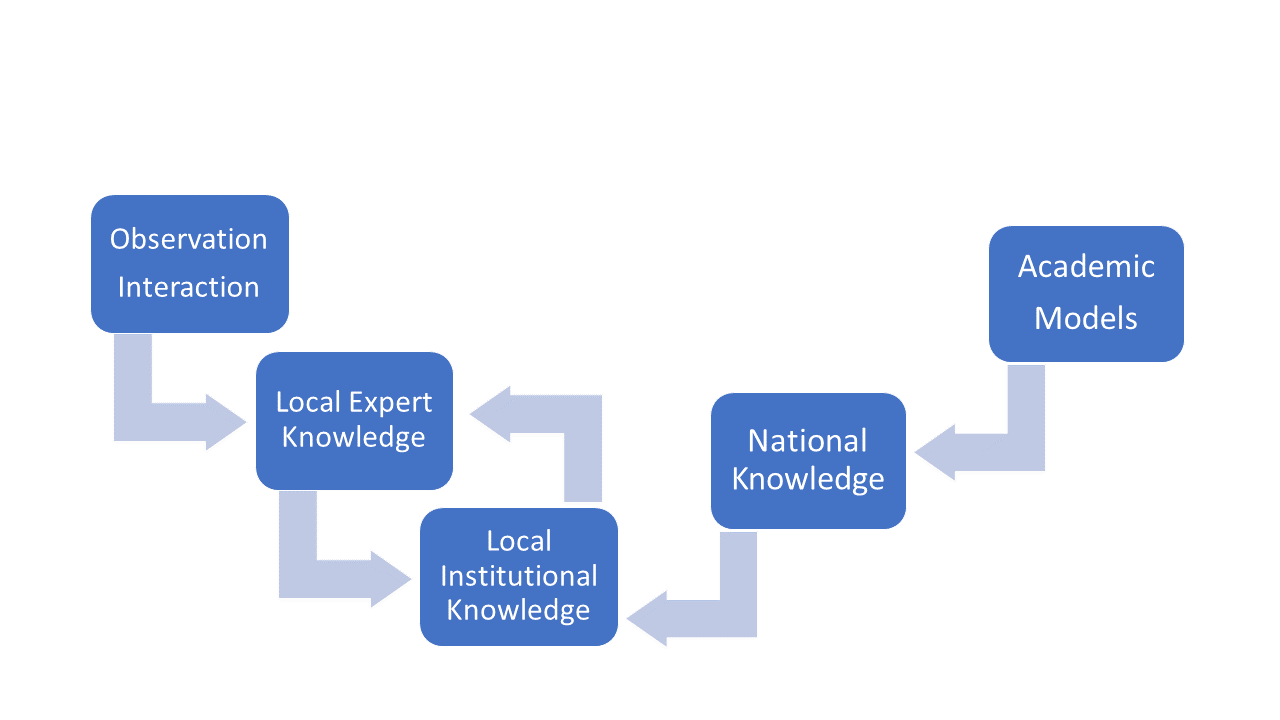
\includegraphics[width=1\textwidth]{fig_theory/local knowledge accumulation.png}

%create figure descriptor in a simple box 
\begin{frame}{Figure Local Knowledge Production. Created using the information stream outlined in \cite{setten_we_2019} and \cite{rod_integrated_2012}}
\end{frame}

As can be seen in figure** above Local Expert knowledge is created as many may assume from local observations and local interactions. Yet, local expert knowledge also is created from local institutional knowledge. This local institutional knowledge is in turn co-produced by local expert knowledge. In this case the local expert knowledge is often considered more informal than the formalised local institutional knowledge, but does not need to be limited to this.  Academic models and national knowledge do feed into local expert knowledge and local institutional knowledge. Yet, their has been highlighted that particularly for disaster risk management the local institutional and expert knowledge doesn't always feedback to these other producers of knowledge\cite{rod_integrated_2012}. The questions about the alignment between local knowledge and academic models of the changing sea level extremes influenced the creation of this project. 

\paragraph{}

Local knowledge is often highlighted as a key facet of community resilience \cite{setten_we_2019}. With the assumption being the higher levels of local knowledge particularly higher levels of awareness about natural systems and natural hazards increases community resilience.  How local knowledge interacts with community resilience and where this belongs in a place-based conceptualisation of resilience is discussed in the social systems of resilience section below. Awareness of local risk is here considered as a facet of local knowledge.  

 
%memory vs awareness vs knowledge 
 
\subsection{Vulnerability}
Vulnerability of a place is impacted by many broad influences including Local Knowledge 
Vulnerability – Lujala / Lein / Setten 



\subsection{Space,Time, Place} 
To understand resilience we must ask resilience: for whom; of what; to what; of where; how and when \cite{cutter_community_2020}, \cite{moser_turbulent_2019}. Resilience is temporally and spatially dynamic \cite{cutter_community_2020}. Hence a basic description of what is meant here by space, time and place is necessary. The conceptualisation used here is inline with \cite{massey_for_2005}, where space is the dimension of simultaneity and is part of space-time. In this view space is considered as the dimension of things being and importantly occurring at the same time. In contrast time is considered as things occurring one after the other. This conceptualisation of space-time is relevant for private, public and even virtual spaces and gives room for the social networks that operate within these spaces \cite{massey_for_2005} \cite{allen_rethinking_1998}.

\paragraph{}
The four chosen research places are created upon a combination of public and private space. The majority of the edge of the water in Norway can be considered public space, but but there is also space allocated to specific groups which can create feelings of in-place vs out-of-place. Place is considered as an assemblage of traces. These traces range from the historical and global to the local and present and it is these combinations of traces which combine to make these places \cite{anderson_understanding_2015} \cite{massey_for_2005}. As well as explicit group membership the traces of place influence who can feel in-place and what is culturally and legally allowable uses of the places \cite{anderson_understanding_2015}. The four research sites include a wide demographic users of who can be considered in-place, but the power relationships and the in-place members affect the resilience of the location. 

\subsection{Awareness}
To understand the current resilience of a place requires an understanding of the awareness of the people who interact with and define the place. An individual’s ability to rank their level of awareness about a subject is a long investigated and debated topic *ref*. It is generally preferable to allow them to display their level of awareness rather than ask them on a sliding scale how aware they are. This is especially important when trying to explore knowledge which may have previously been seen as lesser.

\paragraph{}
To determine awareness level three questions were set in the survey used. These questions were designed to be simple and quick to answer in a format which would allow the author to analyse awareness about sea level extremes in the present and future along with general knowledge of the sea. Awareness about tide level, current risk of storm surges, past resilience to storm surges and future resilience to storm surges was investigated. Further information of how different question techniques and formats were trialled, and the influence of the decided questions format can be found in the Discussion section.

%insert graphic to be the same width as the text
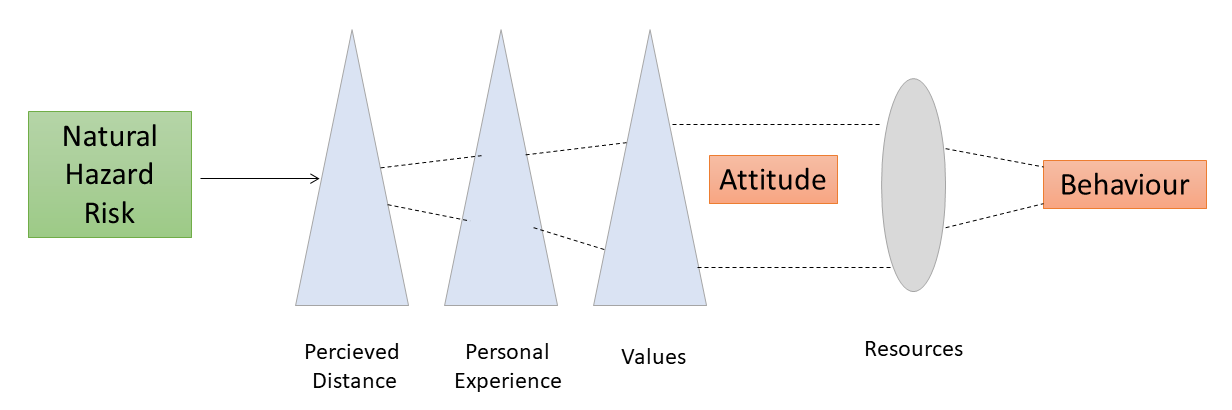
\includegraphics[width=1\textwidth]{fig_theory/awareness lujala and whitmarsh.png}

%create figure descriptor in a simple box 
\begin{frame}{Awareness of Natural Hazard Risk to behaviour pipeline based of \cite{lujala_climate_2015}\cite{whitmarsh_are_2008}.}
\end{frame}

Resilience is impacted by the behaviour of those who are potentially impacted by the potential hazard. Awareness is influenced by many factors. Fig ** above is based on \cite{whitmarsh_are_2008} and \cite{lujala_climate_2015} . Where the green box labelled "Natural Hazard Risk" is the awareness of the individual about the risk. The three triangles are the prisms of "perceived distance", "personal experience" and "values" which have a significant impact on how this awareness is manifested as attitude to the natural hazard risk. This "attitude" is then put through the lens of "resources" before influencing the behaviour of the individual. 
\paragraph{}
Of course people's information in, to thought, to behaviour process are much more complicated than the visualisation above, but it is helpful to considered these prisms and lens when attempting to understand why individuals behave as they do. There is assumptions that those with higher levels of awareness about risks are more likely to have certain attitudes and in turn certain behaviours, but this is not always the case. \cite{lujala_climate_2015}  Awareness of the changing tides and risk of storm surges is considered here as an aspect of local knowledge and is one of the key factors investigated to determine the resilience of Trondheim to sea level extremes. 

\section{Theories Used}
\subsection{Resilience}
Resilience - cutter

\section{Projecting Resilience of Place}

There are many theories on resileince and the term has many varied and wide conceptulisations. 

The concpetulisation here is influence by ....

Key theories:
•	DROP cutter
•	Social systems as what defines resilience
•	Projected resilience as dynamic process which influences outcomes (i.e. resilience as measured post disaster). 
•	Cutter et al 2008
•	Cutter 2020 
•	Moser et al 2019 

\section{Defining Resilience} 
Resilience is here considered as the ability to return to normality as quickly as possible after disaster this is in line with (Cutter, 2019:Löw, 2019).

"present does not define future resilience, but it does influence it. Resilience as dynamic and dependent on 3 changing systems -natural, social and technological
" \cite{cutter_community_2020} views of resilience.

Sea Level Extremes can cause disaster, but this is not necessarily the case. A sea level extreme thus can be viewed as a possible disaster which is referred to here as an event. 

""Resilience is the ability of a social system to respond and recover from disasters and includes those inherent conditions that allow the system to absorb impacts and cope with an event, as well as post-event, adaptive processes that facilitate the ability of the social system to re-organize, change, and learn in response to a threat" "Vulnerability is the pre-event, inherent characteristics or qualities of social systems that create the potential for harm. Vulnerability is a function of the exposure (who or what is at risk) and sensitivity of system (the degree to which people and places can beharmed" " \cite{cutter_place-based_2008}

%insert graphic and rezise 
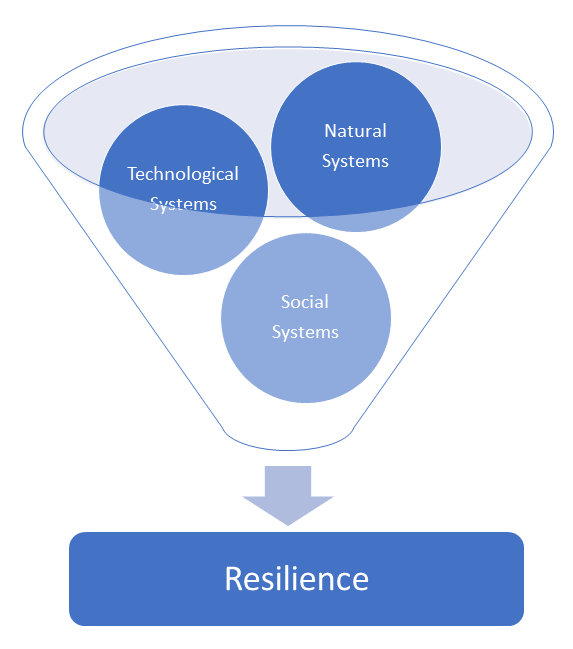
\includegraphics[scale=0.5]{fig_theory/resilience model .png}

%insert graphic to be the same width as the text
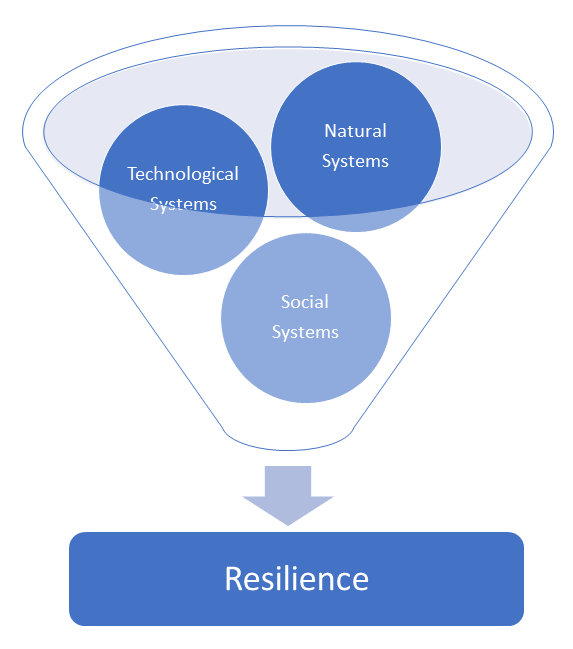
\includegraphics[width=1\textwidth]{fig_theory/resilience model .png}

%create figure descriptor in a simple box 
\begin{frame}{Figure Model of Projected Resilience and the systems involved in its creation }
\end{frame}

Resilience is an ongoing dynamic process. When discussing resilience in this thesis we are discussing projected resilience. Hence what is the projected ability to return to normality as quickly as possible after an sea level extreme event. 
 
Focusing on place based resilience and including community and institutions under the social system aspect
Rather than using community resilience in its place-based approach as commonly conceptualised in Norway both in National and local policy documents and by “layperson” (Räsänen et al 2020). Especially as highlighted by (Räsänen et al 2020) that how useful current place -based metirics are for measuring community resilience and that there is need for other techniques. Hence don’t ignore community but place it under social systems. 
•	Place based resilience vs community resilience
•	What they are why they differ and why I am using place based resilience


\subsection{Social Systems impacting Resilience}
community resilience as key aspect of social systems
local knowledge is part of that

\subsection{Technological Systems}
%altered coastlines
%observation - watching of coastlines - e.g. person falling in notice scheme in trondheim
%infrastructure 
%models of coastlines

\subsection{Natural Systems }
SLE = WAVE + SEA LEVEL + TIDE + STORM SURGES + land movement

Storm Surge
“Storm surges are high water levels in the sea that occur during spring tides in combination with special weather conditions such as low air pressure and strong onshore winds.” According to the kommune (Einar Aassved Hanssen, Marianne Langedal, 2013) – stormflo = storm surge
“Safety against floods and storm surges is regulated by safety classes based on the
largest nominal annual probability. Flood sizes are usually stated with a number of
years of repetition intervals. The recurrence interval indicates how often a flood or
storm surge of the same magnitude occurs on average over many long years. A flood
with a recurrence interval of 200 years, also called a 200-year flood, occurs on average
every 200 years. Each year, the probability of a 200-year flood is equal to 1/200, ie 0.5 percent.
This does not exclude that one can get two 200-year floods at short intervals.
Calculation of recurrence intervals for floods and storm surges is based on historical
observations, and measurement of water flow or water level.”
Building technical regulations (TEK17) with guidance Chapter 7 Safety against natural stresses

\title{Sea Level Extremes}
%insert graphic to be the same width as the text
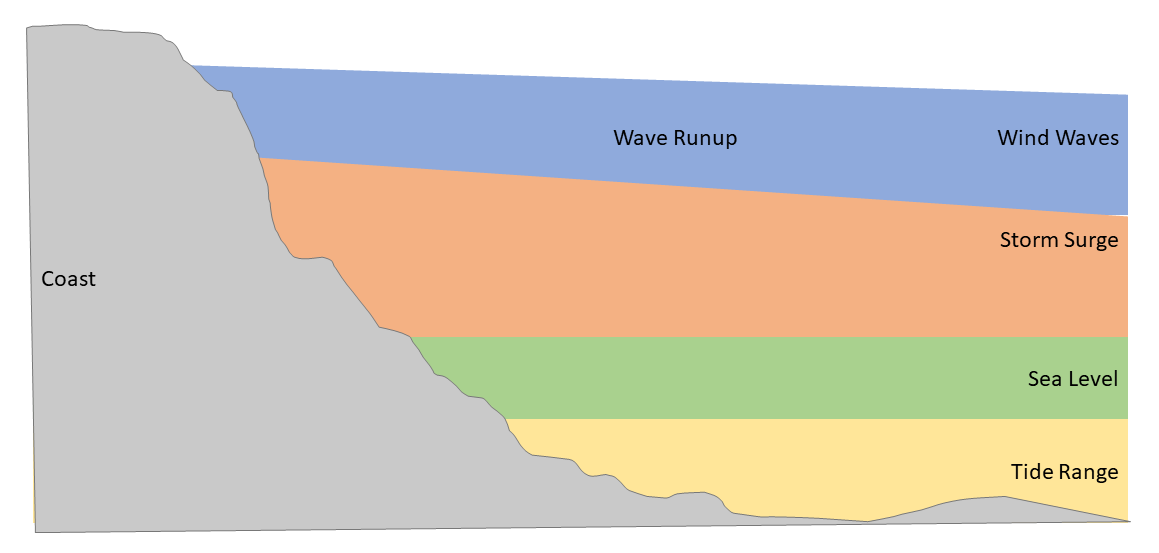
\includegraphics[width=1\textwidth]{fig_theory/sea level extremes.png}

%create figure descriptor in a simple box 
\begin{frame}{Figure The various aspects which combine to create extreme sea levels. Tide Range, Sea Level, Storm Surge, Waves due to the wind, Waves due to the run-up onto the coast.}

Sea Level extremes are due to the combination of various variables which for Trondheim's fjord can be impacted by the changing climate. 

\end{frame}


